%! Licence = CC BY-NC-SA 4.0

%! Author = gianfluetsch, mariuszindel
%! Date = 30. Dez 2021
%! Project = cydef_summary


\section{Mail Security}
DKIM, SPF und DMARC sind Standards, die verschiedene Aspekte der E-Mail-Authentifizierung ermöglichen.
\begin{center}
    \vspace{-8pt}
    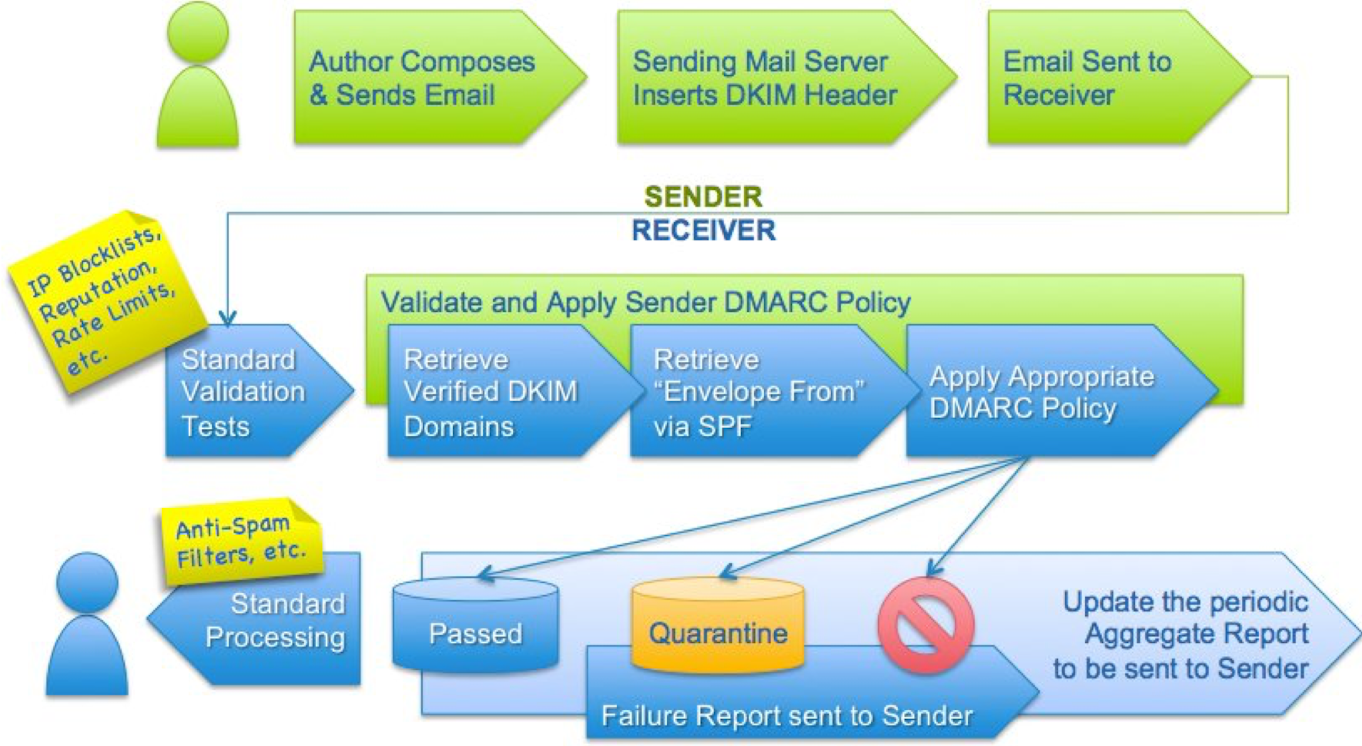
\includegraphics[width=.8\linewidth]{./img/07-mail_security/overview}
    \vspace{-8pt}
\end{center}
\begin{center}
    \vspace{-8pt}
    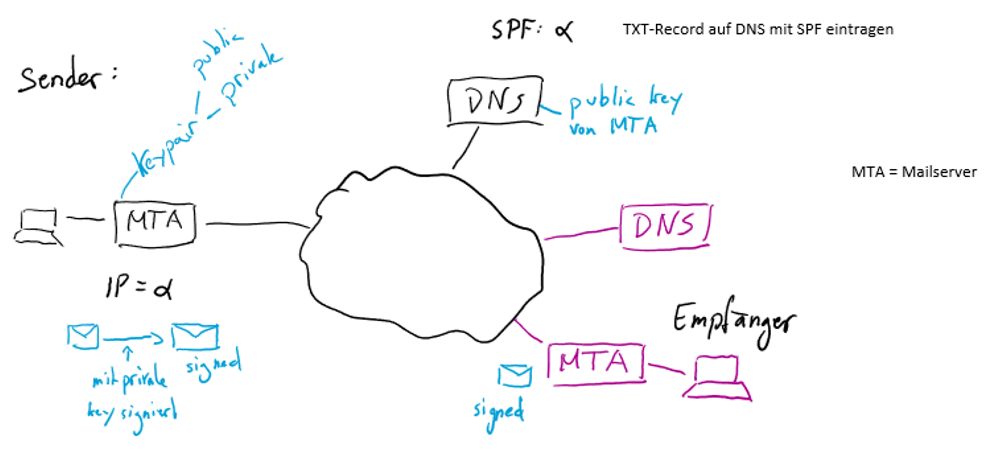
\includegraphics[width=1.0\linewidth]{./img/07-mail_security/spf_overview}
    \vspace{-8pt}
\end{center}

\subsection{SPF: Sender Policy Framework}
Mit SPF können Absender festlegen, welche IP-Adressen E-Mails für eine bestimmte Domäne senden dürfen.

\textit{SPF} ist besonders effizient gegen \textcolor{red}{\textbf{Phishing-Angriffe}}.

\subsubsection{Ablauf}
Auf dem \textbf{DNS} kann eingegrenzt werden, wer (welche IP) alles ein Mail verschicken darf.
\textcolor{purple}{\textbf{MTA}} macht \textbf{DNS-Lookup} und fragt diesen an, welche IPs berechtig sind Mails zu versenden.\\
IP-$\alpha$ (TCP) $\rightarrow$ DNS-Lookup $\rightarrow$ SPF@ost.ch

Wenn Empfänger SPF-Policy nicht enforced, ist egal was der Sender konfiguriert hat. Empfänger-MTA interessiert das nicht.\\

\subsubsection{Header}
Wenn SPF verwendet wird, sollte dies im Header/ Log ersichtlich sein!
\begin{center}
    \vspace{-8pt}
    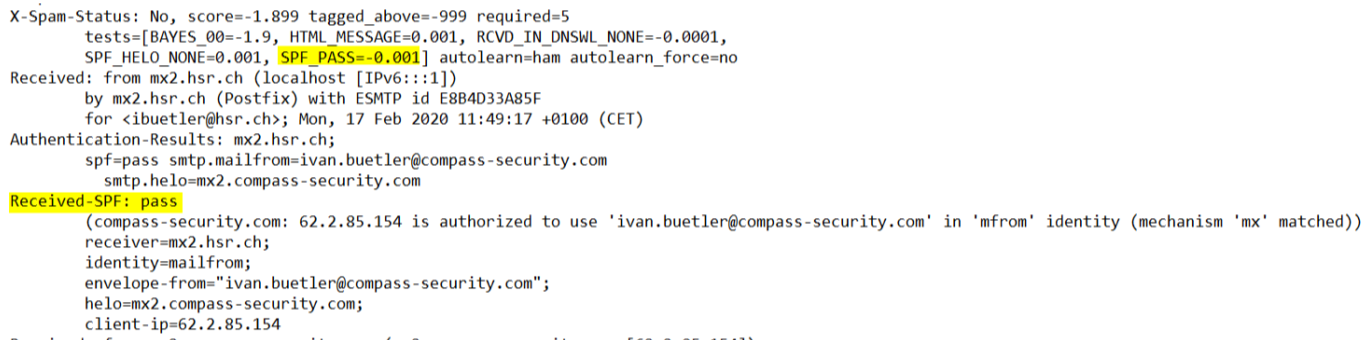
\includegraphics[width=1.0\linewidth]{./img/07-mail_security/spf}
    \vspace{-8pt}
\end{center}
\begin{center}
    \vspace{-8pt}
    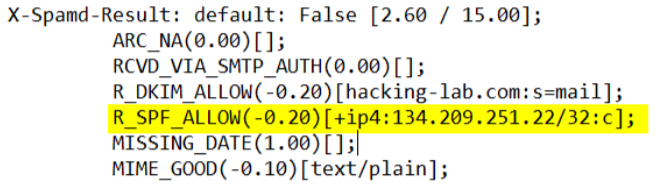
\includegraphics[width=.6\linewidth]{./img/07-mail_security/spf2}
    \vspace{-8pt}
\end{center}
\begin{center}
    \vspace{-8pt}
    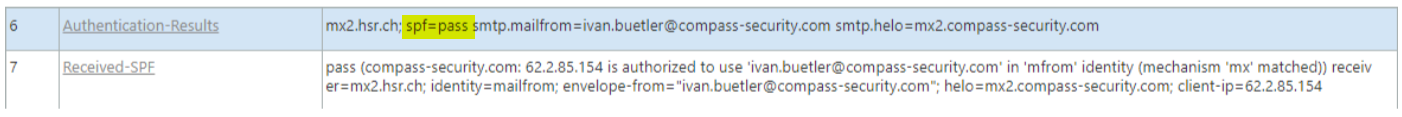
\includegraphics[width=1.0\linewidth]{./img/07-mail_security/spf3}
    \vspace{-8pt}
\end{center}

\subsection{DKIM: DomainKeys Identified Mail}
DKIM stellt einen Verschlüsselungsschlüssel und eine digitale Signatur bereit, mit denen überprüft wird, dass eine E-Mail-Nachricht nicht gefälscht oder verändert wurde.

\textit{DKIM} ist besonders effizient gegen \textcolor{red}{\textbf{Man-in-the-middle-Angriffen}}.

\subsubsection{Ablauf}
\begin{itemize}
    \item Mailserver signiert Mail mit private Key
    \item Mail kommt beim  \textcolor{purple}{MTA} an und dieser prüft ob Mail signiert ist
    \begin{itemize}
        \item Wenn Signatur vorhanden $\rightarrow$ \textbf{DNS-lookup} für public key $\rightarrow$ prüft Signatur von Mail mit dem public key des \textbf{DNS Servers}\\
    \end{itemize}
\end{itemize}

\subsubsection{Header}
Wenn DKIM verwendet wird, sollte dies im Header/ Log ersichtlich sein!
\begin{center}
    \vspace{-8pt}
    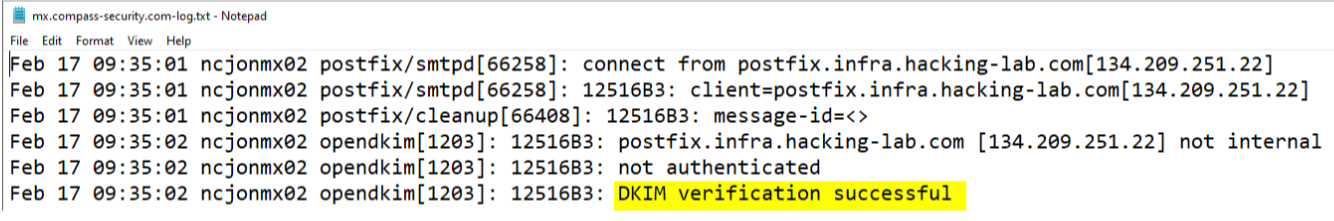
\includegraphics[width=1.0\linewidth]{./img/07-mail_security/dkim}
    \vspace{-8pt}
\end{center}
Due to the MX of Compass, the \textit{DKIM} service is initialized. But the headers from the OWA do not have DKIM headers applied. Thus, DKIM isn't used!
\begin{center}
    \vspace{-8pt}
    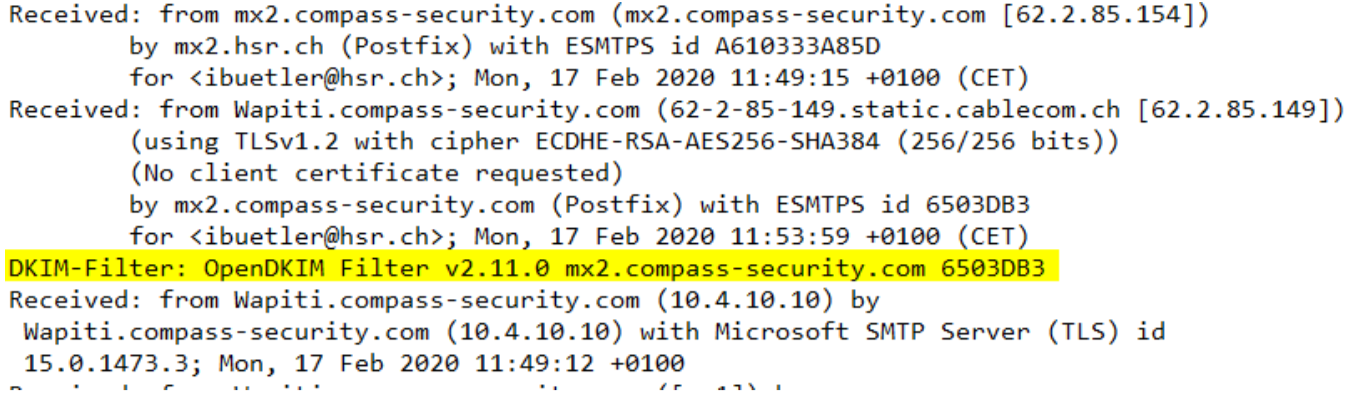
\includegraphics[width=.8\linewidth]{./img/07-mail_security/dkim2}
    \vspace{-8pt}
\end{center}

\subsection{DMARC: (Domain-based Message Authentication, Reporting, and Conformance}
DMARC vereinheitlicht die Authentifizierungsmechanismen SPF und DKIM in einem gemeinsamen Rahmen und ermöglicht es den Inhabern von Domänen zu definieren, wie E-Mails von dieser Domäne behandelt werden sollen, wenn sie einen Autorisierungstest nicht besteht.

DMARC is available!
\begin{center}
    \vspace{-8pt}
    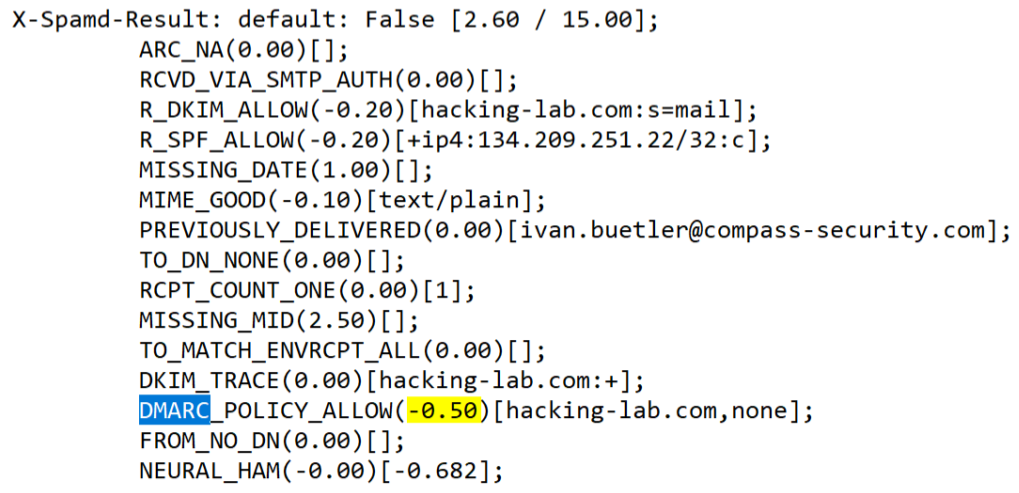
\includegraphics[width=.8\linewidth]{./img/07-mail_security/dmarc}
    \vspace{-8pt}
\end{center}
DMARC not available (NA)!
\begin{center}
    \vspace{-8pt}
    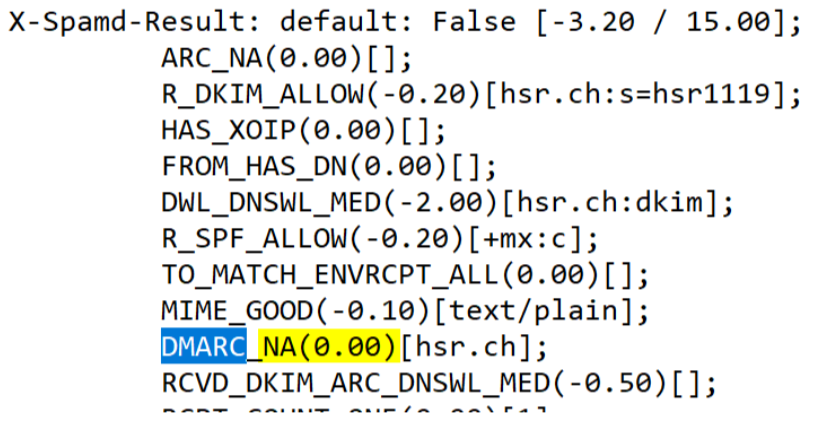
\includegraphics[width=.6\linewidth]{./img/07-mail_security/dmarc2}
    \vspace{-8pt}
\end{center}


%TODO: Can't find this chapter in lecture?
%\subsection{Opportunistic TLS Encryption}
%By checking the pcap files, one can see the \textit{STARTTLS} messages which will let us know tls encryption has been used.
%
%\begin{center}
%    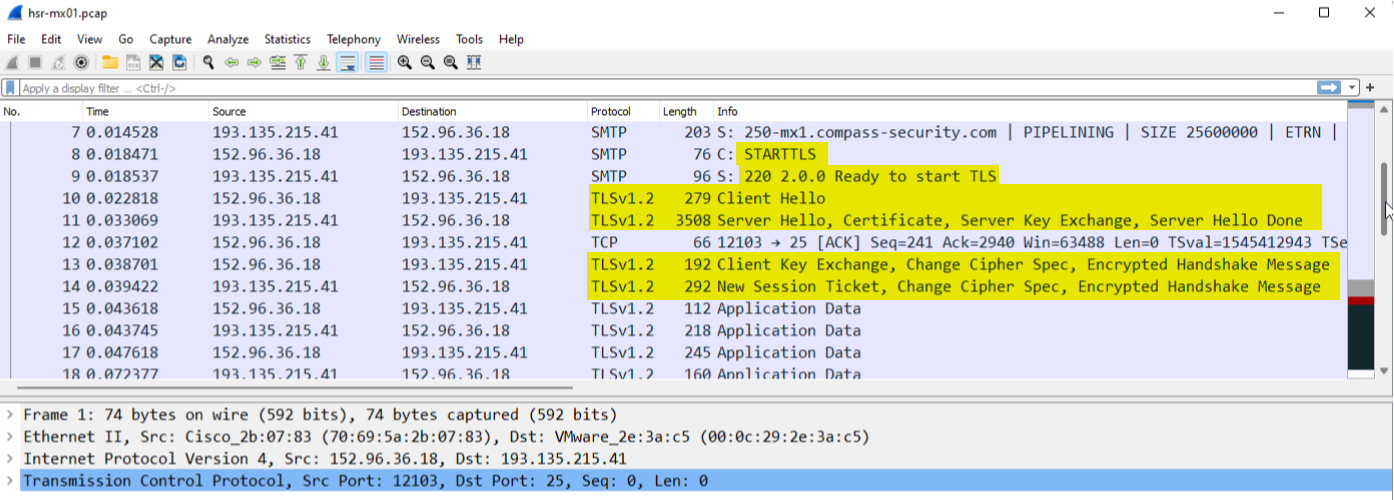
\includegraphics[width=1.0\linewidth]{./img/07-mail_security/tls_encryption}
%\end{center}
%

%
%\subsection{Spam Mails}
% TODO: (mägge)
%
%

